\section{Caso de Teste 3}

Este caso de teste está dividido em 5 (cinco) cenários, os quais são apresentados a seguir, contemplando todo o processo de auto-localização
em cada exemplo, a partir da apresentação das imagens a seguir, Figura \ref{img:cen3_ex1} a Figura \ref{img:real_cen3_ex5}.

\subsection{Cenário 1}

Cenário utilizando velocidade de deslocamento em 2 unidades de diâmetro por segundo:

{\centering
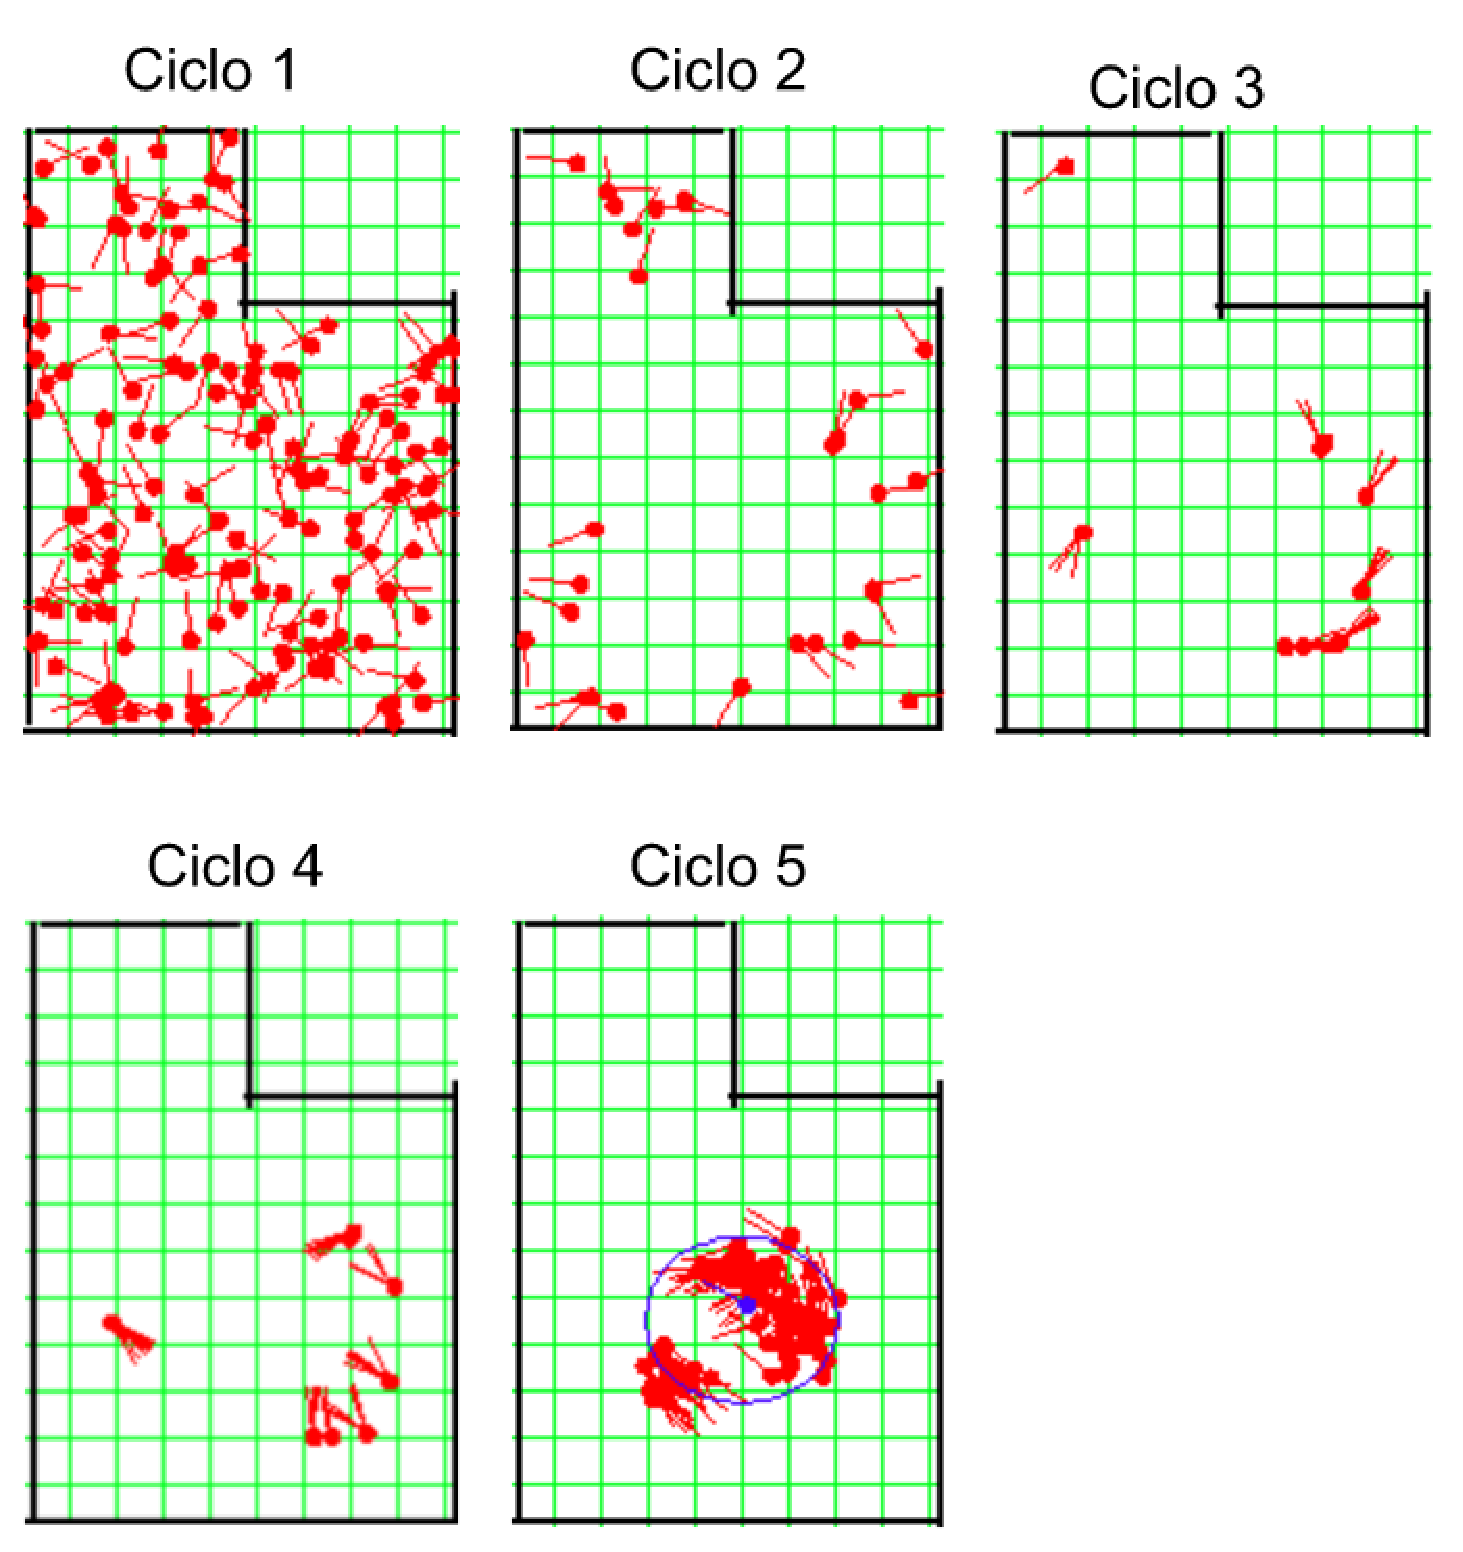
\includegraphics[scale=0.4]{figuras/cen3_ex1.eps}
\captionof{figure}{Caso de Teste 3 - Cenário 1}
\label{img:cen3_ex1}
\par}

{\centering
\includegraphics[scale=0.2]{figuras/real_cen3_ex1.eps}
\captionof{figure}{Posição Real do Caso de Teste 3 - Cenário 1.}
\label{img:real_cen3_ex1}
\par}


\subsection{Cenário 2}

Cenário utilizando velocidade de deslocamento em 5 unidades de diâmetro por segundo:

{\centering
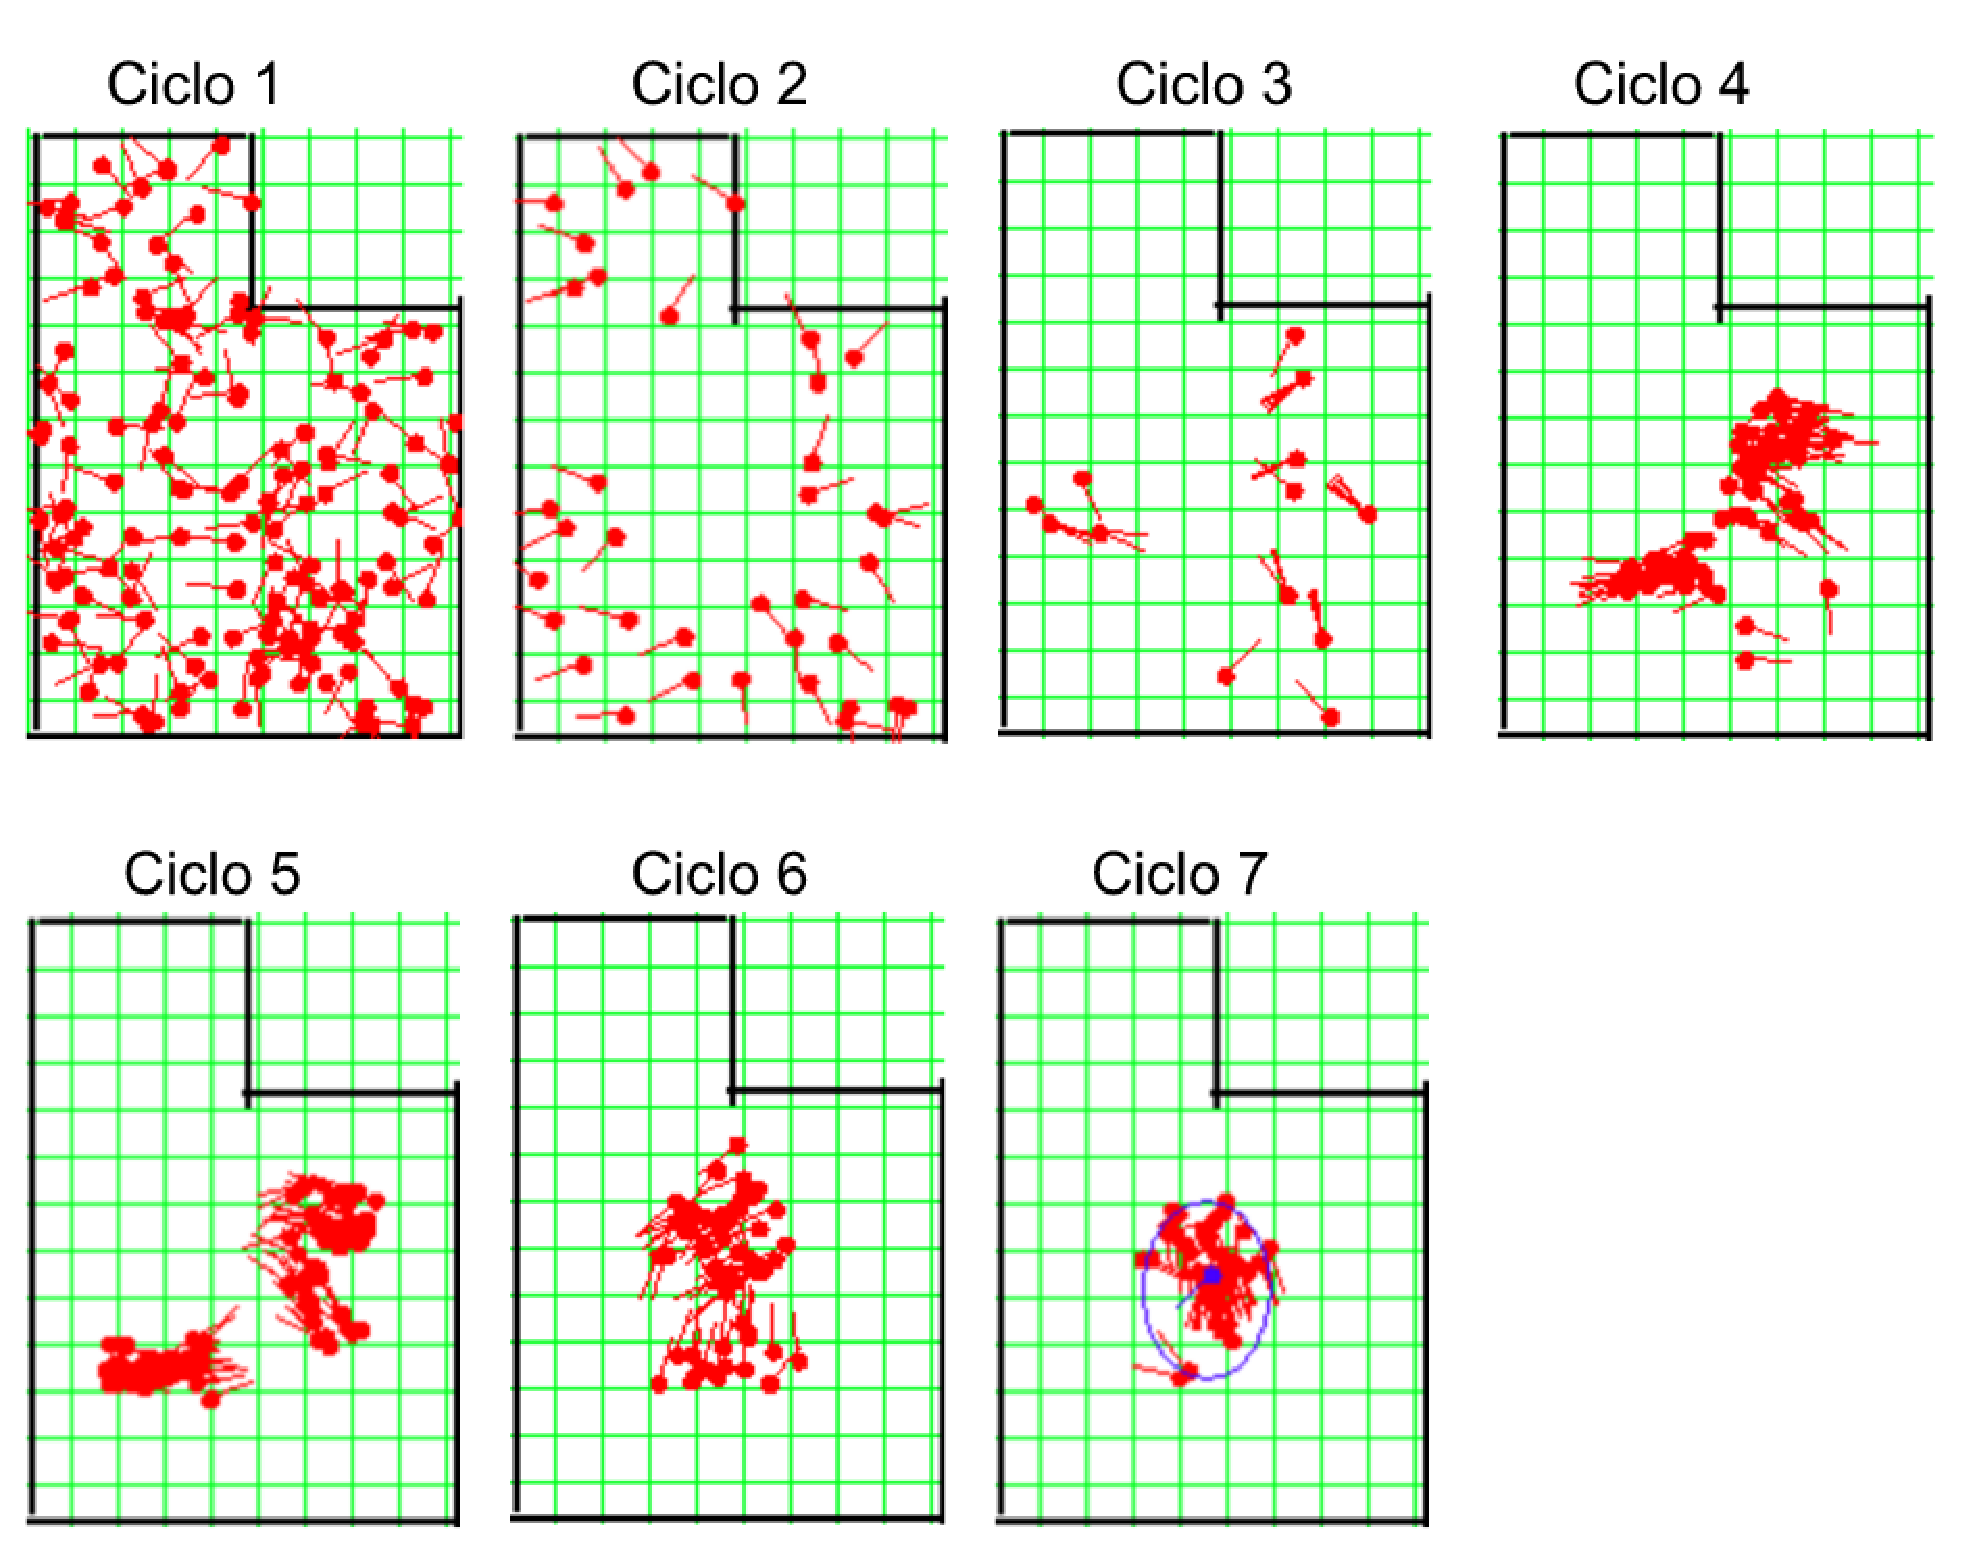
\includegraphics[scale=0.4]{figuras/cen3_ex2.eps}
\captionof{figure}{Caso de Teste 3 - Cenário 2}
\label{img:cen3_ex2}
\par}

{\centering
\includegraphics[scale=0.2]{figuras/real_cen3_ex2.eps}
\captionof{figure}{Posição Real do Caso de Teste 3 - Cenário 2.}
\label{img:real_cen3_ex2}
\par}


\subsection{Cenário 3}

Cenário utilizando velocidade de deslocamento em 10 unidades de diâmetro por segundo:

{\centering
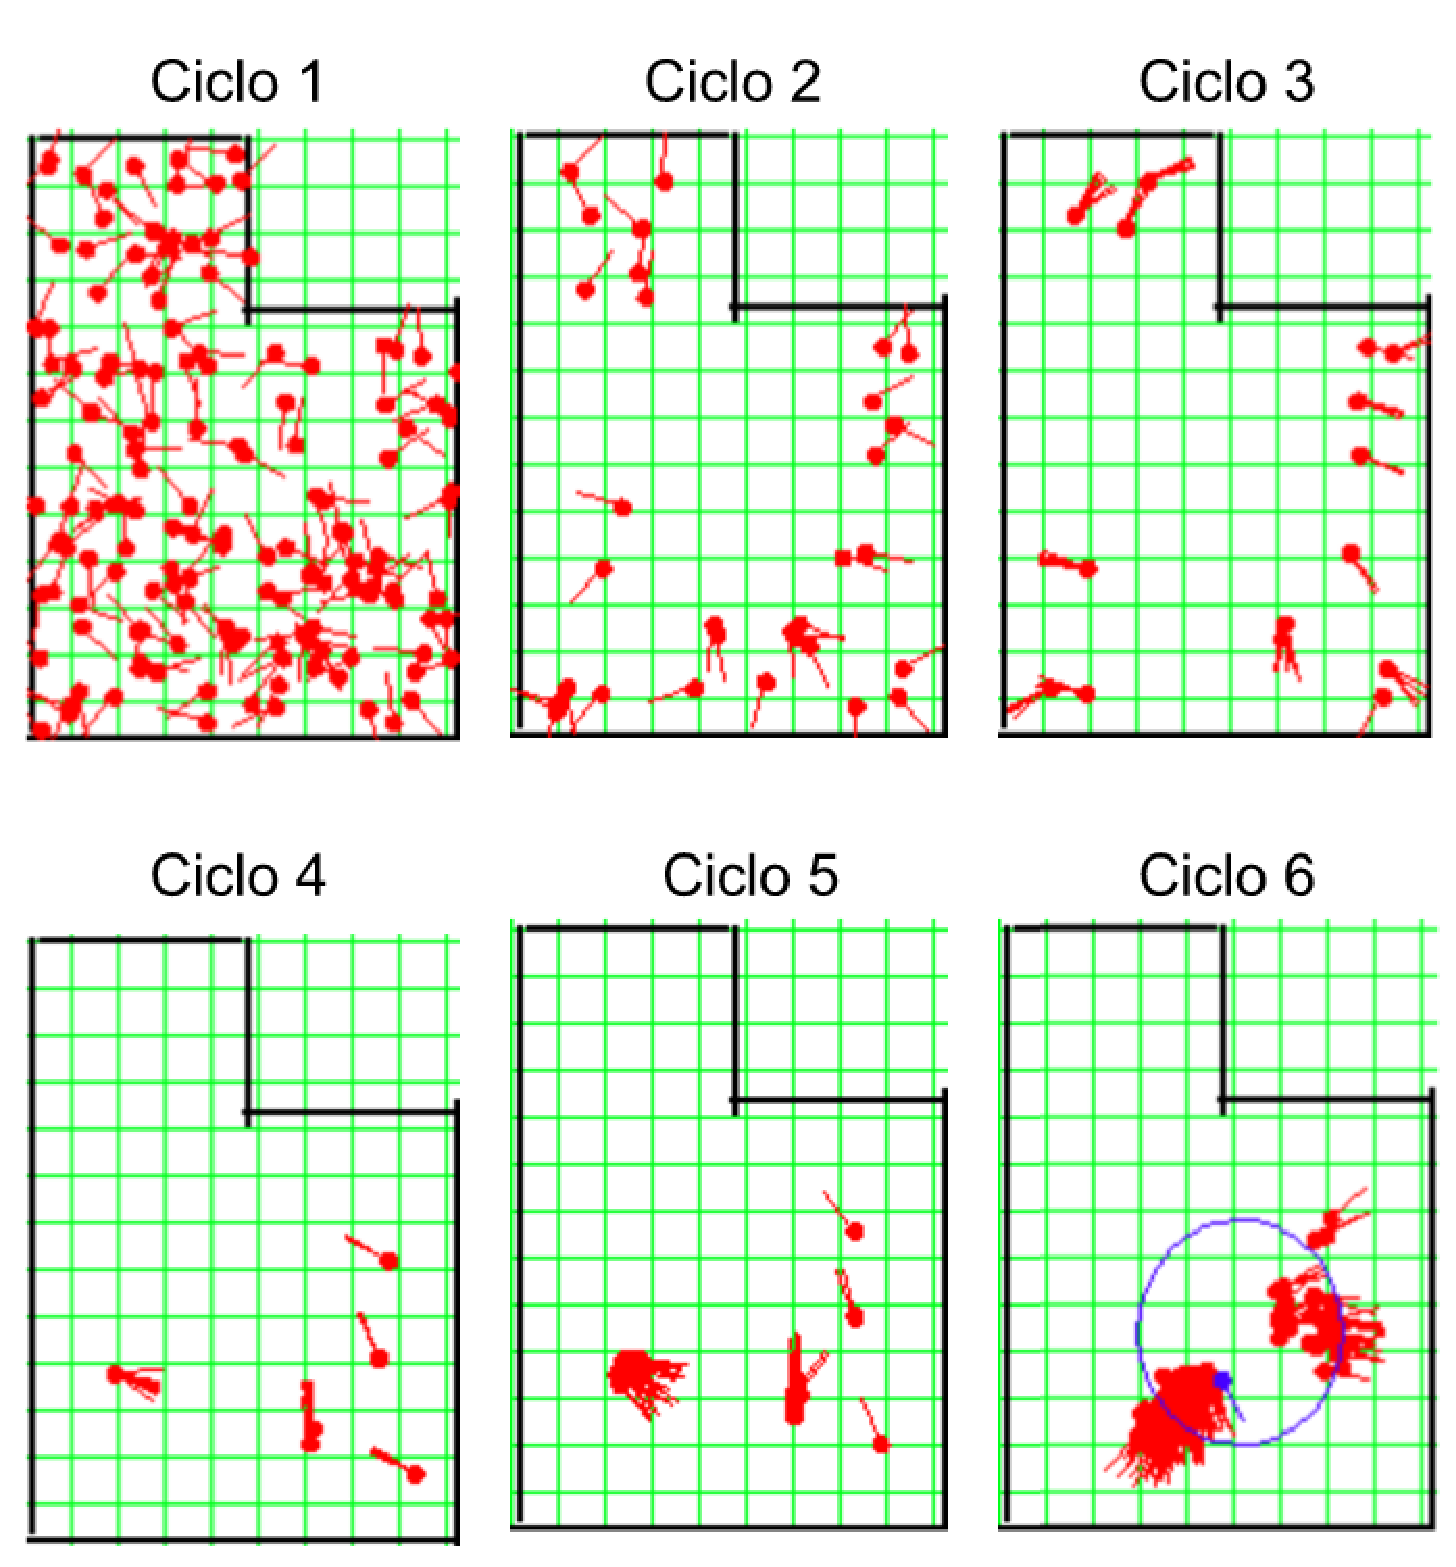
\includegraphics[scale=0.4]{figuras/cen3_ex3.eps}
\captionof{figure}{Caso de Teste 3 - Cenário 3}
\label{img:cen3_ex3}
\par}

{\centering
\includegraphics[scale=0.2]{figuras/real_cen3_ex3.eps}
\captionof{figure}{Posição Real do Caso de Teste 3 - Cenário 3.}
\label{img:real_cen3_ex3}
\par}

\subsection{Cenário 4}

Cenário utilizando velocidade de deslocamento em 15 unidades de diâmetro por segundo:

{\centering
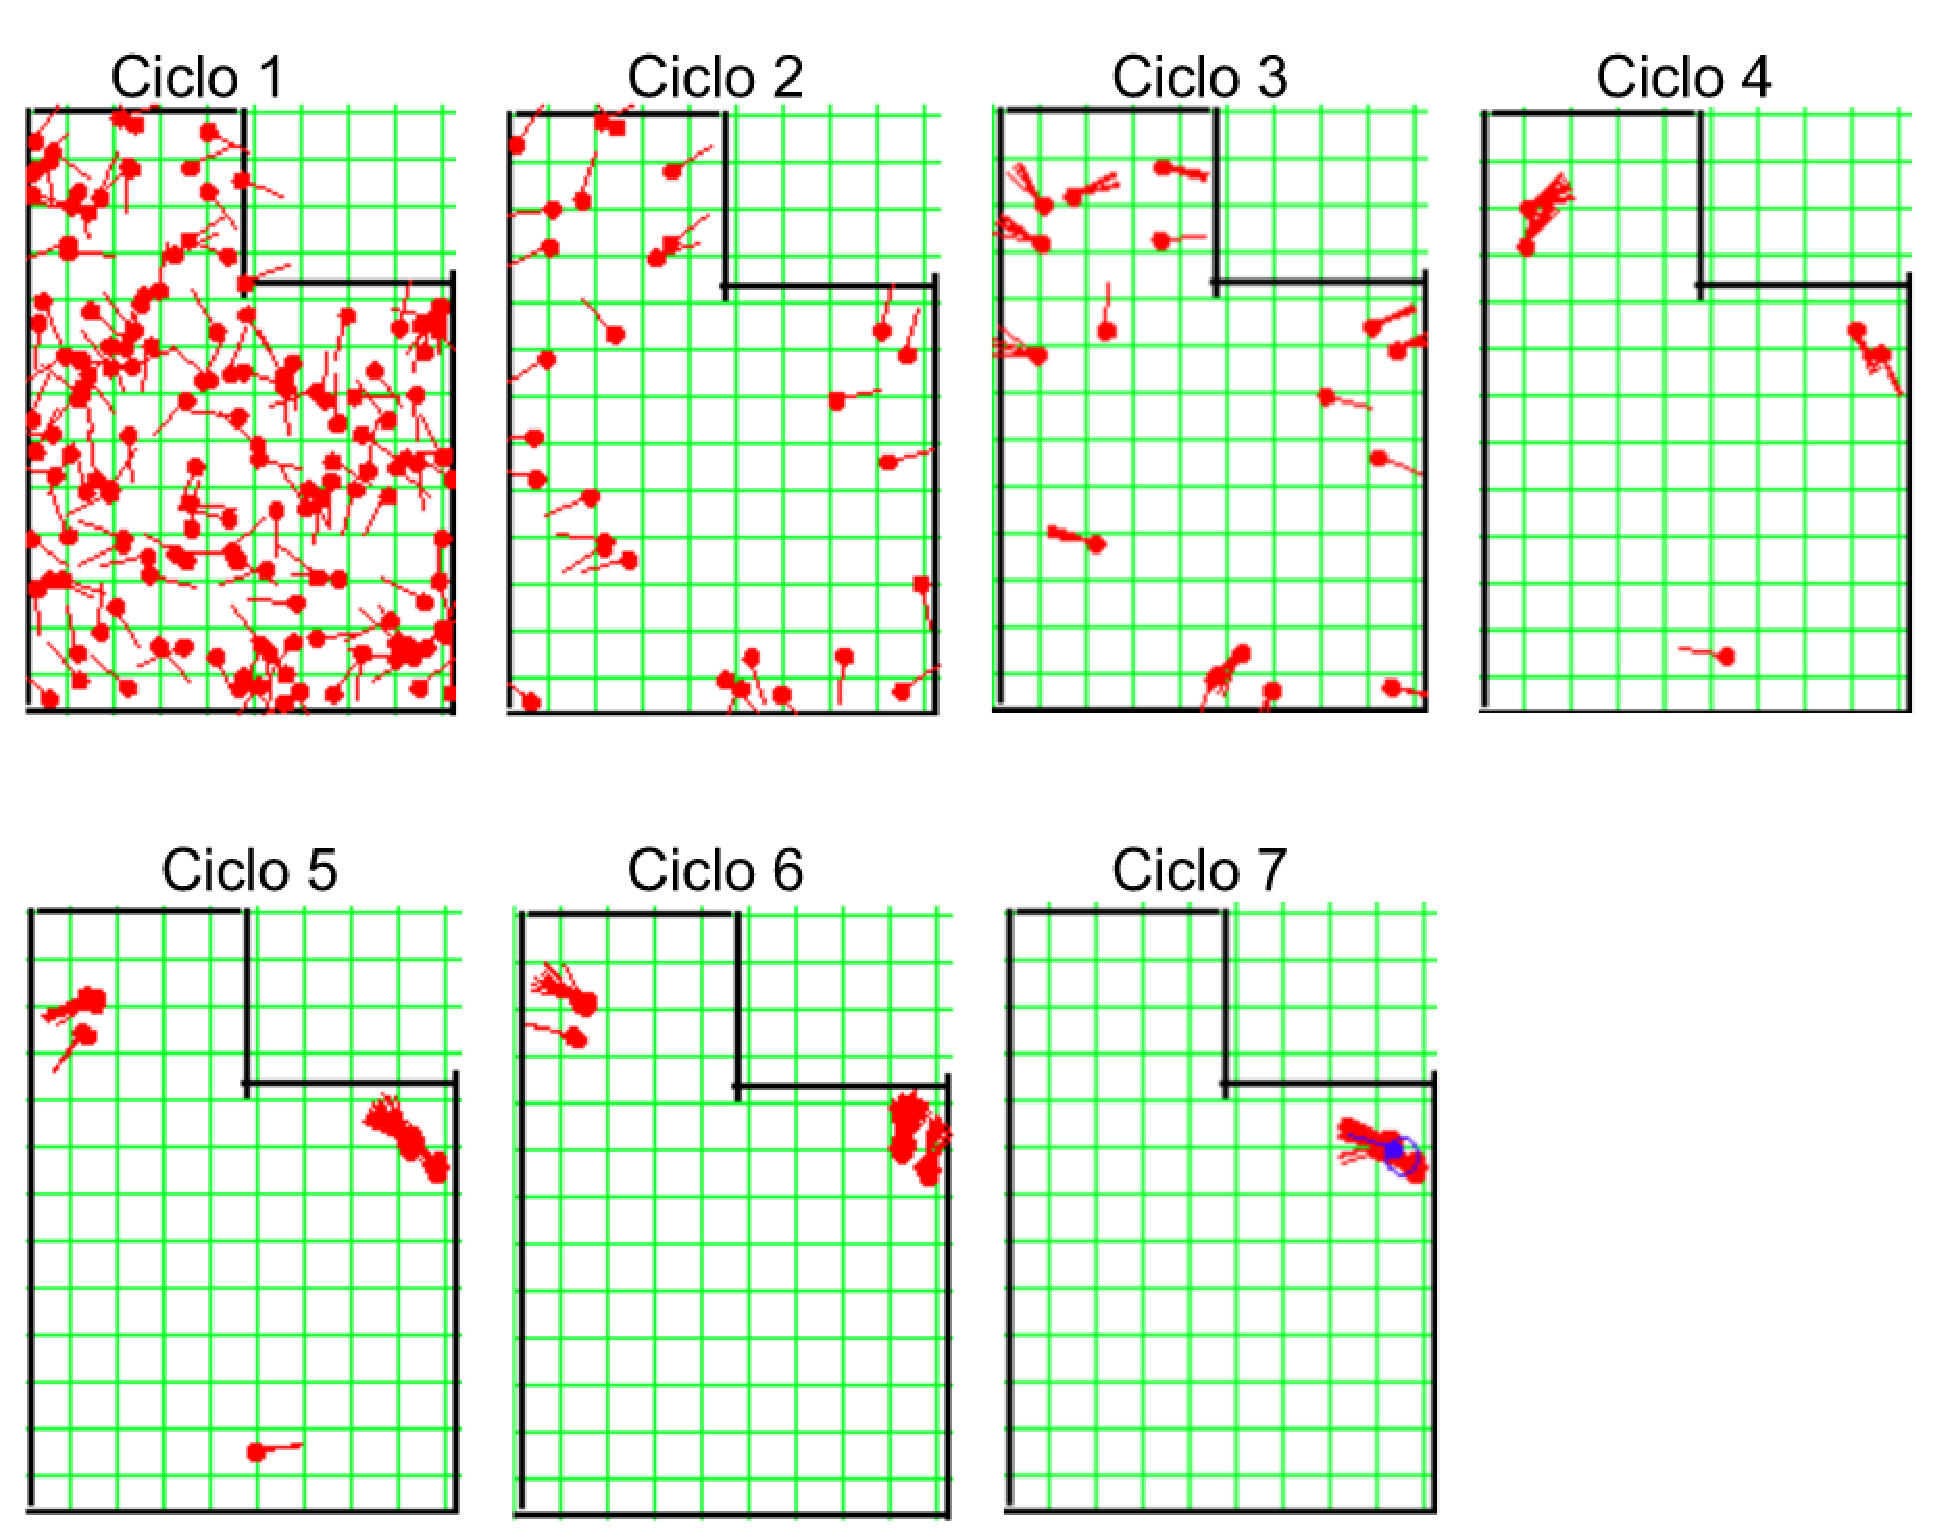
\includegraphics[scale=0.4]{figuras/cen3_ex4.eps}
\captionof{figure}{Caso de Teste 3 - Cenário 4}
\label{img:cen3_ex4}
\par}

{\centering
\includegraphics[scale=0.2]{figuras/real_cen3_ex4.eps}
\captionof{figure}{Posição Real do Caso de Teste 3 - Cenário 4.}
\label{img:real_cen3_ex4}
\par}

\subsection{Cenário 5}

Cenário utilizando velocidade de deslocamento em 30 unidades de diâmetro por segundo:

{\centering
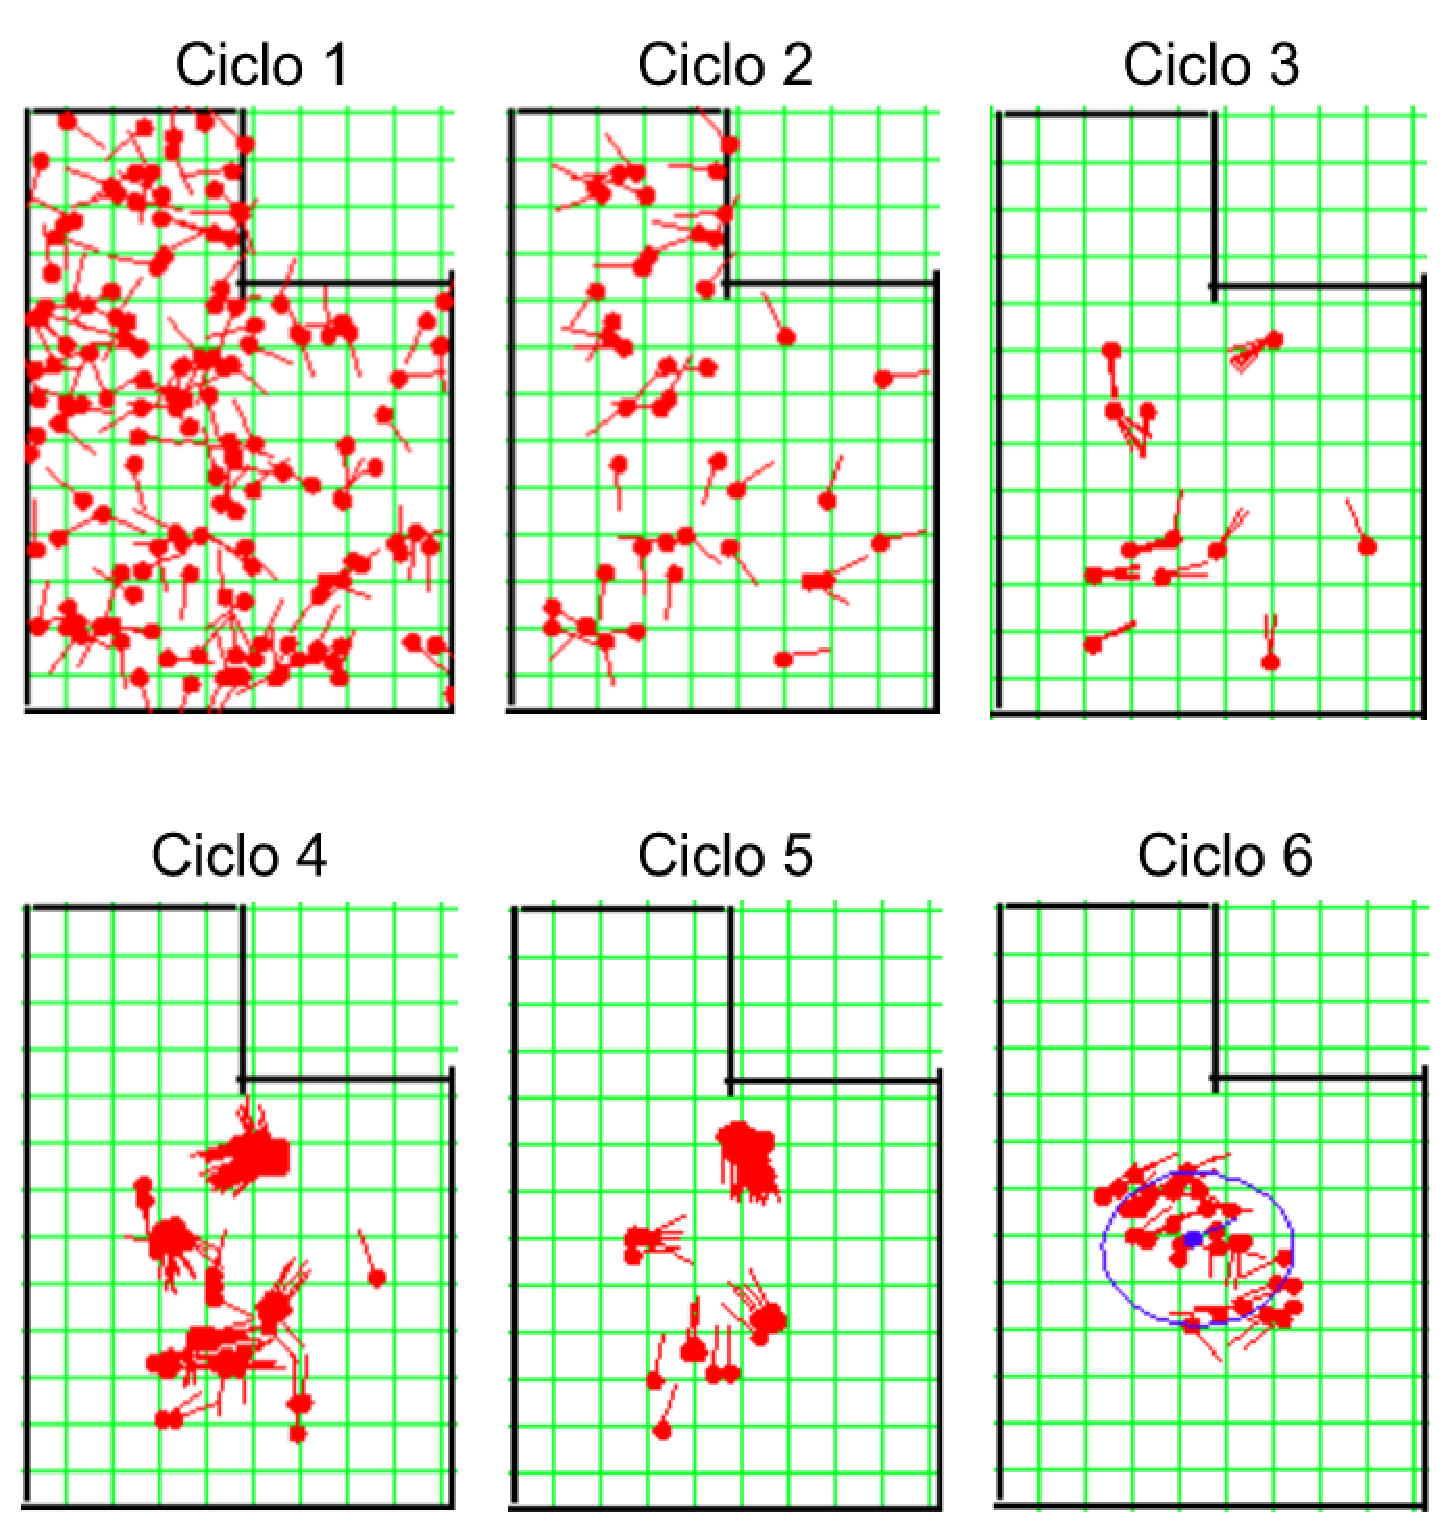
\includegraphics[scale=0.4]{figuras/cen3_ex5.eps}
\captionof{figure}{Caso de Teste 3 - Cenário 5}
\label{img:cen3_ex5}
\par}

{\centering
\includegraphics[scale=0.2]{figuras/real_cen3_ex5.eps}
\captionof{figure}{Posição Real do Caso de Teste 3 - Cenário 5.}
\label{img:real_cen3_ex5}
\par}
